%%%%%%%%%%%%%%%%%%%%%%%%%%%%%%%%%%%%%%%%%%%%%%%%%%%%%
% Preamble
%%%%%%%%%%%%%%%%%%%%%%%%%%%%%%%%%%%%%%%%%%%%%%%%%%%%%

%\documentclass[11pt,table,handout]{beamer}
\documentclass[11pt,table]{beamer}
\input{/Users/dasirianni/Documents/tex_templates/beamer/beamer_preamble.tex}
\usepackage{threeparttablex}
\usepackage{ltablex}

%%%%%%%%%%%%%%%%%%%%%%%%%%%%%%%%%%%%%%%%%%%%%%%%%%%%%
% Themes
%%%%%%%%%%%%%%%%%%%%%%%%%%%%%%%%%%%%%%%%%%%%%%%%%%%%%

\usefonttheme{professionalfonts}

%%%%%     Special Themes     %%%%%

% Georgia Tech
\input{/Users/dasirianni/Documents/tex_templates/beamer/themes/gatech.tex}

%%%%%%%%%%%%%%%%%%%%%%%%%%%%%%%%%%%%%%%%%%%%%%%%%%%%%
% Macros
%%%%%%%%%%%%%%%%%%%%%%%%%%%%%%%%%%%%%%%%%%%%%%%%%%%%%

\input{/Users/dasirianni/Documents/tex_templates/ref_styles.tex}
\input{/Users/dasirianni/Documents/tex_templates/math_macros.tex}

%%%%%%%%%%%%%%%%%%%%%%%%%%%%%%%%%%%%%%%%%%%%%%%%%%%%%
% Title & Author Information
%%%%%%%%%%%%%%%%%%%%%%%%%%%%%%%%%%%%%%%%%%%%%%%%%%%%%

\title[8/27: Advanced Python]{Namespaces, Scope, \&\\
Modules/Packages}

\author[D. A. Sirianni]{D. A. Sirianni}
\institute[GT Chemistry]{CHEM 4803/8843 DR\\$\,$\\
School of Chemistry \& Biochemistry\\ 
Georgia Institute of Technology}
\date{27 August 2019}
\makeatletter
\makeatother

%%%%%%%%%%%%%%%%%%%%%%%%%%%%%%%%%%%%%%%%%%%%%%%%%%%%%
% Title & Outline Frames
%%%%%%%%%%%%%%%%%%%%%%%%%%%%%%%%%%%%%%%%%%%%%%%%%%%%%

\begin{document}

%\titleframe
\GTtitleframe
\frontTOC

%%%%%%%%%%%%%%%%%%%%%%%%%%%%%%%%%%%%%%%%%%%%%%%%%%%%%
% Content Frames
%%%%%%%%%%%%%%%%%%%%%%%%%%%%%%%%%%%%%%%%%%%%%%%%%%%%%

%----------------------------------------------------
\section{Scope \& Namespaces}
\subsection{Primer}
\begin{frame}[fragile]{Primer}

\only<1>{\vspace{-2cm}}
What will the following code, {\tt scope\_test.py}, print?
\begin{mintypython}
some_name = 'Bob'

def print_name():
    some_name = 'Alice'
    print(f'In here, the name is {some_name}')

print(f'Out here, the name is {some_name}')
print_name()
\end{mintypython}

\begin{onlyenv}<2>
Answer:
\begin{mintybash}
$ python scope_test.py

Out here, the name is Bob.
In here, the name is Alice.
\end{mintybash}
\end{onlyenv}

\end{frame}

%----------------------------------------------------
\subsection{Introduction}
\begin{frame}[fragile]{Some Definitions}

\begin{block}{Namespace}
A {\em namespace} is a mapping of name to object, as in a Python dictionary:
\begin{mintypython}
space1 = {'name1': var1, 'name2': var2, ...}
space2 = {'name0': var1, 'name3': var2, 'name4': var4, ...}
\end{mintypython}
Note: Namespaces are completely independent, and their names have no relation
to one another.  Furthermore, they can have different lifetimes.
\end{block}

\begin{block}{Scope}
{\em Scope} is the textual region of a Python program where a namespace is
directly accessible.
\end{block}

\end{frame}

%----------------------------------------------------
\subsection{Scoping: Rules and Precedence}
\begin{frame}[fragile]{Scope Regions: Local \& Global}

\begin{mintypython}
# Here is the global (G) scope
global_var = "This is a global variable"

def my_function():
    # This is the local (L) scope
    local_var = "This is a local variable"
\end{mintypython}

\onslide<2>{
\begin{block}{Namespace Precedence}
When Python searches for the object associated with a particular name, it
proceeds from $L\rightarrow G$; this is referred to as their {\em namespace
precedence}.
\end{block}}

\end{frame}

%----------------------------------------------------

\begin{frame}[fragile]{Scope Regions: Enclosing \& Built-In}

\begin{mintypython}
# Here is the global (G) scope
global_var = "This is a global variable"

def outer_function():
    # This is the enclosing (E) space
    enclosing_var = "This is a nonlocal variable"

    def inner_function():
        # This is the local (L) space
        local_var = "This is a local variable"

# Some names are built-in (B) to Python
print(type(global_var))

def type():
    print("typetypetypetype")

type()
\end{mintypython}

\end{frame}

%----------------------------------------------------

\begin{frame}[fragile]{Namespace Precedence: The LEGB Rule}

\begin{mintypython}
def set():
    def do_local():
        spam = "local spam"
    def do_nonlocal():
        nonlocal spam
        spam = "nonlocal spam"
    def do_global():
        global spam
        spam = "global spam"
    spam = "test spam"
    do_local()
    print("After local assignment:", spam)
    do_nonlocal()
    print("After nonlocal assignment:", spam)
    do_global()
    print("After global assignment:", spam)

set()
print("In global scope:", spam)
\end{mintypython}

\end{frame}

%----------------------------------------------------

\begin{frame}[fragile]{Namespace Precedence: The LEGB Rule}

\begin{mintybash}
$ python legb.py

After local assignment: test spam
After nonlocal assignment: nonlocal spam
After global assignment: nonlocal spam
In global scope: global spam
\end{mintybash}

\onslide<2>{
\begin{block}{The LEGB Rule}
Object namespaces have the following order of precedence:
\begin{center}
Local $\rightarrow$ Enclosed $\rightarrow$ Global $\rightarrow$ Built-In
\end{center}
this is referred to as the {\em LEGB Rule}.
\end{block}}

\end{frame}

%----------------------------------------------------
\section{Code Organization}
\subsection{Primer}
\begin{frame}[fragile]{Organizing Code}

Let's pretend we work for Google Maps. (cool, right?)\\

We have written the following code to compute the distance between two points,
$(x_1, y_1)$ and $(x_2, y_2)$ in Cartesian space:
\begin{mintypython}
def distance(coords1, coords2):
    total = 0.0
    for k in list(len(coords1)):
        total += (coords1[k] - coords2[k]) ** 2
    return (total ** 0.5)
\end{mintypython}

Our colleague wants to write a different function called {\tt distance()} which
takes user input for selecting the points on a map and returns the distance
between them.\\
\end{frame}

%----------------------------------------------------
\begin{frame}[fragile]{Organizing Code}

What are some possible ways she could do this?\\ (Hint: Just think about code
components, not how to actually collect the user input, etc.)

\begin{itemize}
\item Copy our function within her function
\item Copy code from our function directly into hers, don't bother defining
new function
\end{itemize}

\end{frame}

%----------------------------------------------------
\begin{frame}[fragile]{}

\begin{block}{Function-ception!}
\begin{mintypython}
def distance(user_click_1, user_click_2):
    # Our distance function, copied and pasted here
    def distance(coords1, coords2):
        total = 0.0
        for k in list(len(coords1)):
            total += (coords1[k] - coords2[k]) ** 2
        return (total ** 0.5)

    # Colleague's code to collect user clicks
    # and convert latitude-longitude to (x, y)
    ...
    user_cart1 = [user_x_1, user_y_1]
    user_cart2 = [user_x_2, user_y_2]
    cartesian_distance = distance(user_cart1, user_cart2)
    
    # Colleague's code to convert from (x, y) distance to map distance
    ...
    return map_distance
\end{mintypython}
\end{block}

\end{frame}

%----------------------------------------------------
\subsection{Modules \& Packages}
\begin{frame}[fragile]{Modules: A Better Solution}

Instead of literally copying-and-pasting each others' code into the same file,
Python allows us to better organize our code by splitting it up into different
files, called {\em modules}. A collection of modules is called a {\em
package}.\\

If we save our distance function inside a file called {\tt module\_test.py},
our colleague can use our code by {\em importing} our module:
\begin{mintypython}
# Most simple
import module_test

# Give our module a nickname
import module_test as mod

# Import a particular function from our module
from module_test import distance

# Import everything from module_test into current file; just like copy-paste
from module_test import *
\end{mintypython}

\end{frame}

%----------------------------------------------------
\begin{frame}[fragile]{Using Modules}

%\only<1>{\vspace{-2.75cm}}
\begin{block}{Modular Solution}
\begin{mintypython}
def distance(user_click_1, user_click_2):
    # Our distance function, imported and used here
    from module_test import distance

    # Colleague's code to collect user clicks
    # and convert latitude-longitude to (x, y)
    ...
    user_cart1 = [user_x_1, user_y_1]
    user_cart2 = [user_x_2, user_y_2]
    cartesian_distance = distance(user_cart1, user_cart2)
    
    # Colleague's code to convert from (x, y) distance to map distance
    ...
    return map_distance
\end{mintypython}
\end{block}

\end{frame}

%----------------------------------------------------

\begin{frame}[fragile]{After a few months of development...}

\begin{mintypython}
def distance(user_click_1, user_click_2):
    # Our distance function, imported and used here
    from module_test import distance
    ...
    cartesian_distance = distance(user_cart1, user_cart2)
    ...
    return map_distance

def similarity_score(feature_1, feature_2):
    # Convert features to Cartesian coordinates
    ...
    # Compute the distance using our function
    from module_test import distance

    cartesian_distance = distance(feature_cart_1, feature_cart_2)
    ...
\end{mintypython}

\end{frame}

%----------------------------------------------------
\subsection{Module Namespaces}
\begin{frame}[fragile]{Colleague Refactors Her Code...}

Wouldn't it be easier to only import {\em module\_test} once?

\begin{mintypython}
# Our distance function, imported once and used often
from module_test import distance

def distance(user_click_1, user_click_2):
    ...
    cartesian_distance = distance(user_cart1, user_cart2)
    ...

def similarity_score(feature_1, feature_2):
    ...
    cartesian_distance = distance(feature_cart_1, feature_cart_2)
    ...
\end{mintypython}

What problems have we introduced here?

\end{frame}

%----------------------------------------------------
\begin{frame}[fragile]{}

\begin{block}{Module Namespaces}
Each module has its own namespace when it is imported, unless otherwise specified:
\begin{mintypython}
import module            # Imports module as separate namespace
import module as mod     # Gives module namespace a nickname 
from module import func  # Imports function `func` into current namespace
from module import *     # Imports everything into current namespace
\end{mintypython}

Module namespaces can be accessed using ``dot syntax:''
\begin{mintypython}
import module as mod

# Call function `func` from inside `module`'s namespace
result = mod.func()
\end{mintypython}
\end{block}

\end{frame}

%----------------------------------------------------
\begin{frame}[fragile]{Refactored Code Preserving Namespaces}

\begin{mintypython}
# Our module, imported as its own namespace
import module_test as mod

def distance(user_click_1, user_click_2):
    ...
    cartesian_distance = mod.distance(user_cart1, user_cart2)
    ...

def similarity_score(feature_1, feature_2):
    ...
    cartesian_distance = mod.distance(feature_cart_1, feature_cart_2)
    ...
\end{mintypython}

\end{frame}

%----------------------------------------------------

\section{Scientific Computing in Python}
\subsection{Overview}
\begin{frame}{}

\begin{block}{Scientific Computing...}
...is a rapidly growing, multidisciplinary field that uses advanced computing
capabilities to understand and solve complex problems. It is an area of science
which spans many disciplines, but at its core it involves the development of
models and simulations to understand natural systems.\footnotemark[1]
\end{block}

\begin{itemize}
\item Using industry-specific, fully-featured programs 
\item Integrating existing/available tools to solve specific problems 
\item Writing custom software routines to perform simulations, etc.
\end{itemize}

\footnotetext[1]{From Wikipedia, article ``Computational Science.''
\url{https://en.wikipedia.org/wiki/Computational_science}}
\end{frame}

%----------------------------------------------------
\begin{frame}{Python Libraries for Scientific Computing}

\vfill
\begin{itemize}
\item SciPy: Diverse capabilities for scientific computing
\vfill
\item NumPy: Numerical linear algebra routines
\vfill
\item Pandas: Database capabilities
\vfill
\item Scikits: Domain-specific tools in a variety of fields
\vfill
\item Matplotlib: Generates publication-quality plots \& figures
\vfill
\item Keras \& Tensorflow: Neural Networks made easy!
\vfill
\item Many others: \url{https://wiki.python.org/moin/NumericAndScientific}
\end{itemize}
\vfill

\end{frame}

%----------------------------------------------------
\subsection{Research Case Study}
\begin{frame}{An Illustrative Case Study: Curve Minima Interpolation}

\begin{center}
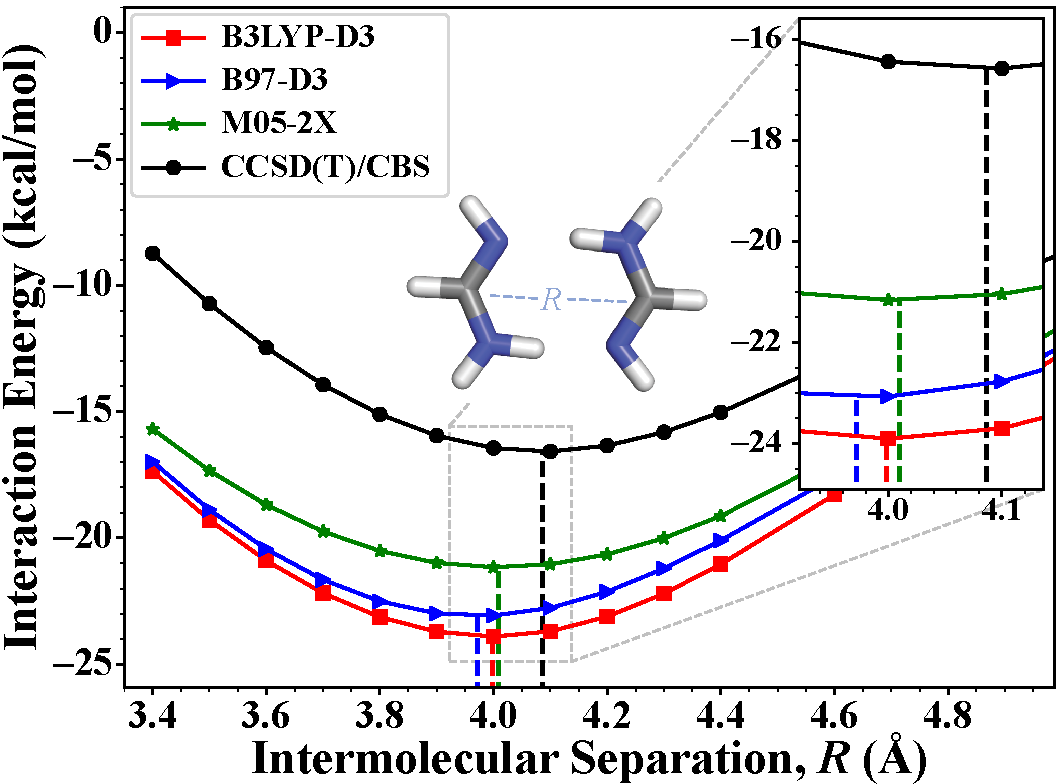
\includegraphics[width=0.8\textwidth]{includes/figure4.pdf}
\end{center}

\end{frame}
%----------------------------------------------------
%\section{Programming Approaches}
%\subsection{Procedural Programming}
%\begin{frame}{Programming Approaches}
%
%\begin{block}{Procedural Programming}
%A style of programming where simple instructions and even functions are
%combined in logical order to execute a given task.
%\end{block}
%
%A procedural approach is best suited for: 
%\begin{itemize}
%\item simple programs, which have a defined purpose not intended for use in
%other contexts or together with other software.
%\end{itemize}
%
%\begin{block}{Object-Oriented Programming (OOP)}
%A style of programming where code is organized into logical containers, called
%{\em objects}, which can be reused in a variety of contexts and by other
%software.
%\end{block}
%
%An object-oriented approach is best suited for: 
%\begin{itemize}
%\item Organizing complicated software, where the objects can be used to carry
%data between software components, or to
%\item Preserve local variable structure.
%\end{itemize}
%
%\end{frame}


%%%%%%%%%%%%%%%%%%%%%%%%%%%%%%%%%%%%%%%%%%%%%%%%%%%%%
% Appendices
%%%%%%%%%%%%%%%%%%%%%%%%%%%%%%%%%%%%%%%%%%%%%%%%%%%%%

%\siTOC

\end{document}
